\documentclass[9pt,twocolumn,twoside,]{pnas-new}

%% Some pieces required from the pandoc template
\providecommand{\tightlist}{%
  \setlength{\itemsep}{0pt}\setlength{\parskip}{0pt}}

% Use the lineno option to display guide line numbers if required.
% Note that the use of elements such as single-column equations
% may affect the guide line number alignment.


\usepackage[T1]{fontenc}
\usepackage[utf8]{inputenc}


\templatetype{pnasresearcharticle}  % Choose template

\title{Culture in oranzees}

\author[a,1]{Alberto Acerbi}
\author[b]{William Snyder}
\author[b]{Claudio Tennie}

  \affil[a]{Centre for Culture and Evolution, Department of Life Sciences, Brunel
University London, Uxbridge, UB8 3PH, United Kingdom}
  \affil[b]{Faculty of Science, Department for early prehistory and quaternary
ecology, University of Tübingen, Schloß Hohentuebingen, Burgsteige 11,
72070, Tübingen, Germany}


% Please give the surname of the lead author for the running footer
\leadauthor{Acerbi}

% Please add here a significance statement to explain the relevance of your work
\significancestatement{Authors must submit a 120-word maximum statement about the significance
of their research paper written at a level understandable to an
undergraduate educated scientist outside their field of speciality. The
primary goal of the Significance Statement is to explain the relevance
of the work in broad context to a broad readership. The Significance
Statement appears in the paper itself and is required for all research
papers.}


\authorcontributions{Please provide details of author contributions here.}

\authordeclaration{Please declare any conflict of interest here.}


\correspondingauthor{\textsuperscript{} }

% Keywords are not mandatory, but authors are strongly encouraged to provide them. If provided, please include two to five keywords, separated by the pipe symbol, e.g:
 \keywords{  one |  two |  optional |  optional |  optional  } 

\begin{abstract}
Please provide an abstract of no more than 250 words in a single
paragraph. Abstracts should explain to the general reader the major
contributions of the article. References in the abstract must be cited
in full within the abstract itself and cited in the text.
\end{abstract}

\dates{This manuscript was compiled on \today}
\doi{\url{www.pnas.org/cgi/doi/10.1073/pnas.XXXXXXXXXX}}

\begin{document}

% Optional adjustment to line up main text (after abstract) of first page with line numbers, when using both lineno and twocolumn options.
% You should only change this length when you've finalised the article contents.
\verticaladjustment{-2pt}

\maketitle
\thispagestyle{firststyle}
\ifthenelse{\boolean{shortarticle}}{\ifthenelse{\boolean{singlecolumn}}{\abscontentformatted}{\abscontent}}{}

% If your first paragraph (i.e. with the \dropcap) contains a list environment (quote, quotation, theorem, definition, enumerate, itemize...), the line after the list may have some extra indentation. If this is the case, add \parshape=0 to the end of the list environment.

\acknow{Please include your acknowledgments here, set in a single paragraph.
Please do not include any acknowledgments in the Supporting Information,
or anywhere else in the manuscript.}

Intro here

\section*{Materials and methods}\label{materials-and-methods}
\addcontentsline{toc}{section}{Materials and methods}

We built an individual-based model that reproduces a world inhabited by
six populations of ``oranzees'', an hypothetical ape species. The model
is space-explicit: the oranzees populations are located at relative
positions analogous to the six chimpanzees sites in (1). This is
important to determine the genetic predispositions and ecological
availabilities associated to their behaviours (see below). Population
sizes are also taken from the sites in (1). Following (2), we use data
from (3), and we define population sizes as \(N=\{20;42;49;76;50;95\}\).

Oranzees are subject to an age-dependent birth/death process. A time
step \(t\) of the simulation represents a month in oranzees' life. From
when they are 25 years old (\(t=300\)), there is a 1\% probability an
oranzee will die each month, or they die when they are 60 years old
(\(t=720\)). The number of individuals in the population is fixed, so
each time an oranzee dies is replaced by a newborn.

A newborn oranzee does not have any behaviour. Behaviours can be
innovated at each time step. The process of innovation is influenced by:
(i) the oranzees `state', which depends from the behaviours an
individual already possesses, (ii) the frequency of the behaviours
already present in the population (``socially-mediated innovation''),
and (iii) the genetic propensity and ecological availability associated
to the behaviour. At the beginning of the simulations, the populations
are randomly initialised with individuals between 0 and 25 years old.

\subsection*{State}\label{format}
\addcontentsline{toc}{subsection}{State}

In the oranzees world, 64 behaviours are possible. Behaviours are
divided in two categories, namely 32 social and 32 food-related
behaviours.

In the case of social behaviours, we assume four sub-categories of
behaviours, each with eight possible different behaviours, that serve
the same goal. Oranzees' state is based on how many of the four goals
are fulfilled. A goal is considered fulfilled if an oranzee has at least
one behaviour out of the eight in the sub-category. An oranzee has a
state value of \(0.25\) if, for example, has at least one behaviour
among the first eight behaviour, and none of the others, and a state
value of \(1\) if there is at least one behaviour in each sub-category.
\(p_\text{state}\), the probability to innovate a social behaviour, is
drawn from a normal distribution with mean equal to \(1-state\).

Food-related behaviours are also divided in sub-categories, with the
differences that there is a variable number of behaviours in each
sub-category, and that sub-categories are associated to two different
`nutrients'. The idea is that individuals need to balance their
nutritional intake, so that their optimal diet consist in a roughly
equal number of foodstuff for one and the other nutrient. The state, for
food-related behaviours, depends on the total amount of food \emph{and}
on the balance between nutrients, and it is calculated as the sum of
each sub-category fulfilled (as above, for this there needs to be at
least one behaviour) minus the difference between the number of
sub-categories providing nutrient Y and the number of sub-categories
providing nutrient Z. As above, all is normalised between \(0\) and
\(1\), and \(p_\text{state}\) is then calculated (more details in SI).

\subsection*{Socially-mediated innovation}\label{format}
\addcontentsline{toc}{subsection}{Socially-mediated innovation}

At each time step, any oranzees has a probability of innovation for
social and food-related behaviours equal to \(p_\text{state}\) as
described above. The specific behaviour an oranzee will innovate depends
both on the frequency of the behaviours already present in the
population, and on the ecological availability and genetic propensity
associated to the behaviour. A further parameter of the model, \(S\),
controls the probability that each innovation is socially-mediated. When
an innovation is socially-mediated, each behaviour has a probability to
be innovated drawn from a normal distribution with mean equals to its
total instances in the population. When the innovation is not
socially-mediated, the probability of innovating each behaviour is
random. Only one behaviour per category can be innovated at each time
step.

\subsection*{Genetic propensity and ecological
availability}\label{format}
\addcontentsline{toc}{subsection}{Genetic propensity and ecological
availability}

The behaviour selected in the previous step is actually innovated
according to its genetic propensity and, in case of food-related
beahviours, ecological availability.

Genetic propensity is a probability \(p_g(0,1)\), assigned independently
to each of the 64 behaviours. A parameter of the model, \(\alpha_g\),
determines the probability that the genetic propensity of each behaviour
is equal for all the six populations or is different.

If is equal, \(p_g\) is randomly drawn. If different, we assign it using
a geographical gradient. For each behaviour, we choose a random point
and calculate its distance to each population. Distances are then
transformed to \(p_g\) by rescaling them between 0 and 1, so that for
the farther population \(p_g=0\) i.e.~the associated behaviour will be
impossible to express (see SI). Notice that \(\alpha_g=0\) does not mean
that there are not genetic influences on the behaviours, but that there
are no \emph{differences} between the populations with this respect.

Ecological availability is a probability \(p_e(0,1)\) that represents
the likelihood of finding a resource, or its nutritional value, in each
site. Ecological availability is assigned only to food-related
behaviours, and it is calculated in the same way of \(p_g\), using the
parameter \(\alpha_e\) to determine the probability of ecological
availability being different in the six populations.

\subsection*{Model's output}\label{format}
\addcontentsline{toc}{subsection}{Model's output}

We run simulation for \(t_\text{max}=6000\) (corresponding to 500 years
of oranzee-time). For each simulation, following (1), we classify each
behaviour, in each population, as:

\begin{itemize}
\item
  \emph{customary}: a behaviour observed in over 50\% of individuals in
  at least one age class (see SI).
\item
  \emph{habitual}: a behaviour observed in at least two individuals over
  all the population.
\item
  \emph{present}: a behaviour observed in at least one individual over
  all the population.
\item
  \emph{absent}: a behaviour never observed.
\item
  \emph{ecological explanations} is a behaviour that is absent because
  of local ecological features (i.e., in our model, associated to
  \(p_e=0\)).
\end{itemize}

Notice the last category in (1) (\emph{unknown}, i.e. ``the behaviour
has not been recorded, but this may be due to inadequacy of relevant
observational opportunities'') does not apply in our case.

Finally, we calculate the same ``patterns'' described in (1):

\begin{itemize}
\item
  \emph{A}: patterns absent at no site.
\item
  \emph{B}: patterns not achieving habitual frequencies at any site.
\item
  \emph{C}: patterns for which any absence can be explained by local
  ecological factors.
\item
  \emph{D}: patterns customary or habitual at some sites yet absent at
  others, with no ecological explanation, i.e.~the behaviours defined as
  ``cultural''.
\end{itemize}

\section*{Results}\label{results}
\addcontentsline{toc}{section}{Results}

We are particularly interested in the realistic parameter conditions of
moderate to high environmental variability (\(\alpha_e=(0.5,1)\)) and
zero to moderate genetic difference (\(\alpha_g=(0,0.5)\)). We run 20
simulations for each combination (for all, innovation is
socially-mediated, i.e. \(S=1\)). The results show that various
combinations of parameters produces a number of ``cultural'' behaviours
(pattern \emph{D}) consistent with the 38 found in (1), in absence of
any explicit copying mechanism implemented (see Figure \ref{Figure1}).

\begin{figure*}[h!]
\begin{center}
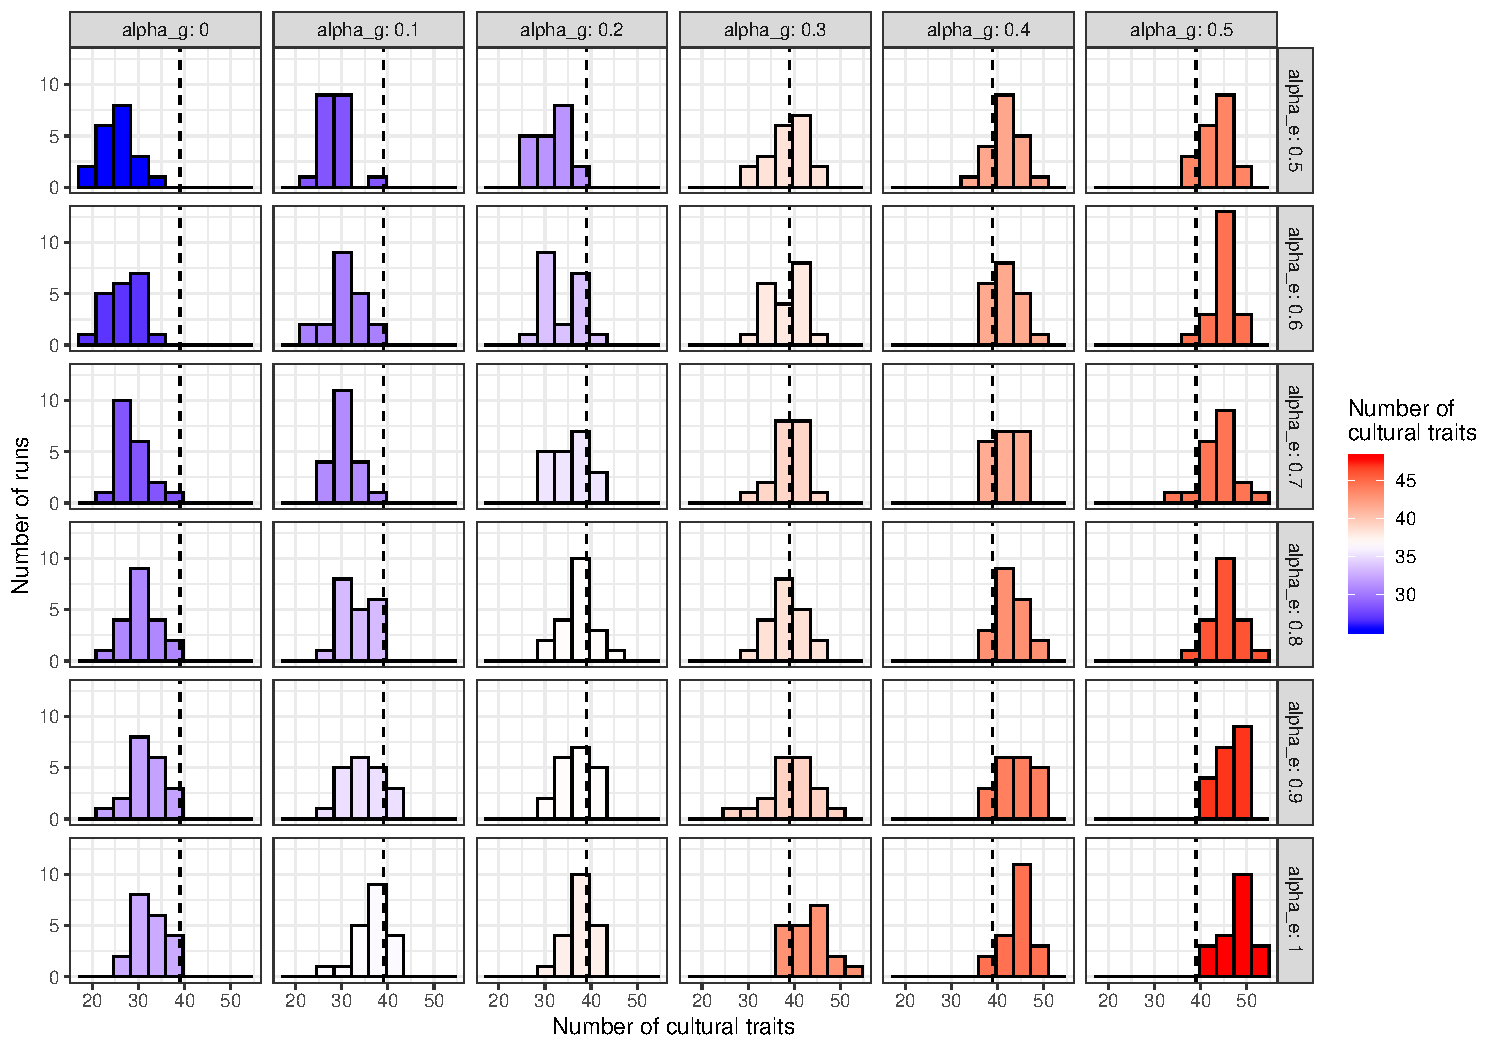
\includegraphics[width=17.8cm]{figures/figure_1.pdf}
\caption{Cultural behaviours in oranzees, varying ecological and genetic diversity. Red colour indicates simulation runs that produced more than 38 cultural behaviours; blue colour indicates simulation runs that produces less than 38 cultural behaviours.}
\label{Figure1}
\end{center}
\end{figure*}

We also analyse the effect of the parameter \(S\) (proportion of
socially-mediated innovations), in three conditions (see Figure
\ref{Figure2}: (a) no genetic differences and intermediate ecological
differences (compare to the high-left angle of Figure \ref{Figure1},
where with \(S=1\) simulations produce less than 38 cultural
behaviours), (b) good match with (1), and (c) intermediate genetic
differences and high ecological differences (compare to the low-right
angle of Figure \ref{Figure1}, where with \(S=1\) simulations produce
more than 38 cultural behaviours). As expected, decreasing \emph{S},
decreases the number of cultural behaviours, so that conditions where
with \(S=1\) there were more than 38 cultural behaviours could still
produce results analogous to (1), if not all innovations are socially
mediated.

\begin{figure*}[h!]
\begin{center}
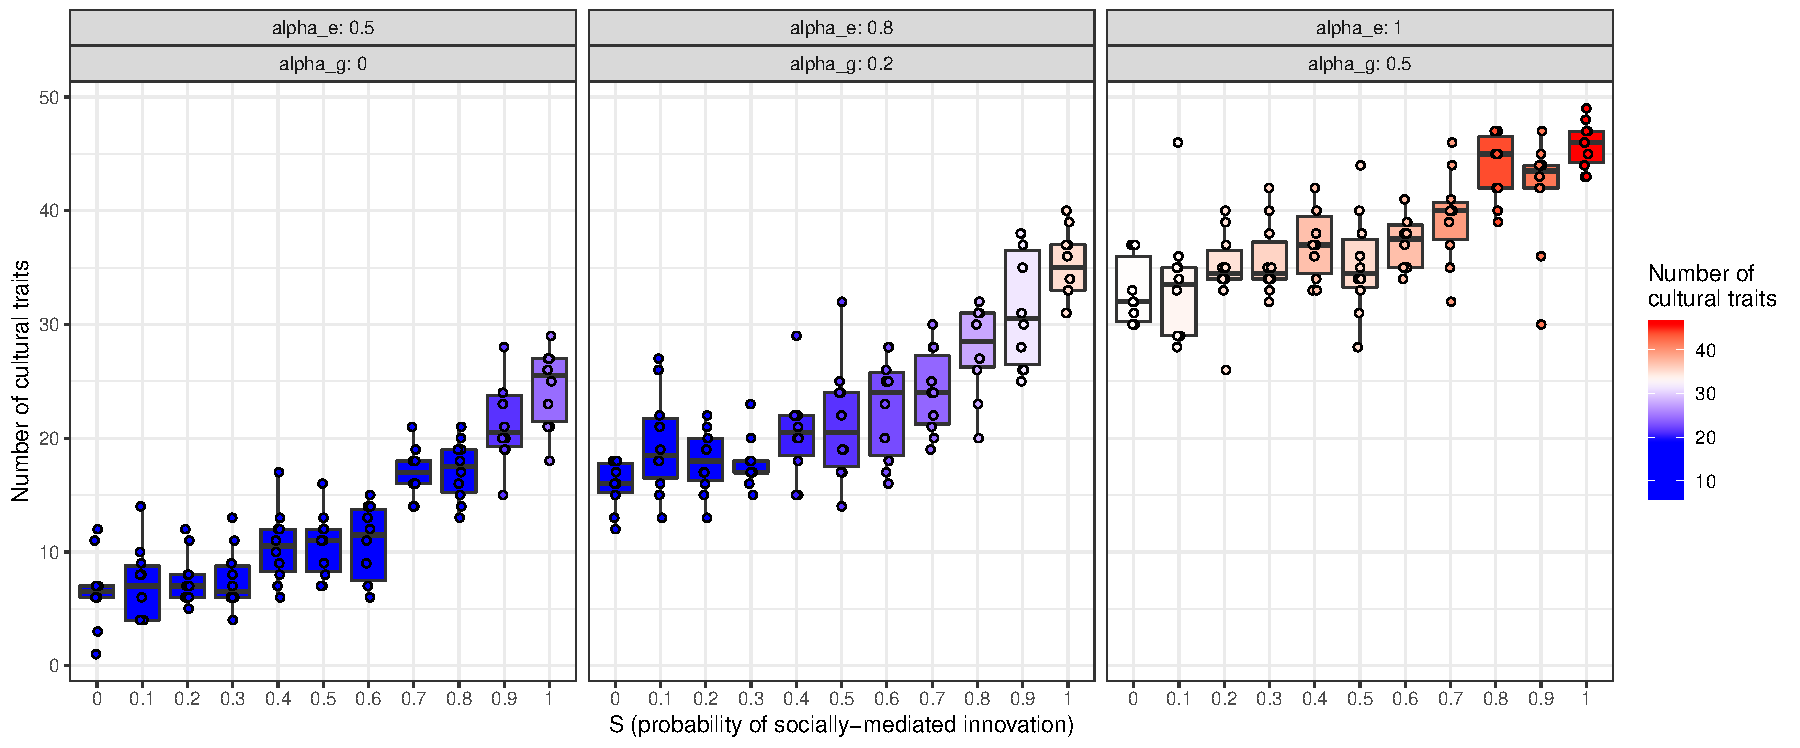
\includegraphics[width=17.8cm]{figures/figure_2.pdf}
\caption{Cultural behaviours in oranzees, varying the probability of socially-mediated innovations. Red colour indicates simulation runs that produced more than 38 cultural behaviours; blue colour indicates simulation runs that produces less than 38 cultural behaviours.}
\label{Figure2}
\end{center}
\end{figure*}

Our results show that our model not only reproduces the number of
cultural behaviours (pattern \emph{D}), but also the other three
patterns (\emph{A}, \emph{B}, \emph{C}) found in (1). Figure
\ref{Figure3} show the four patterns produced in one of the conditions
for which we have a good match for cultural behaviours
(\(\alpha_e=0.8;\alpha_g=0.2, S=1\)).

\begin{figure*}[h!]
\begin{center}
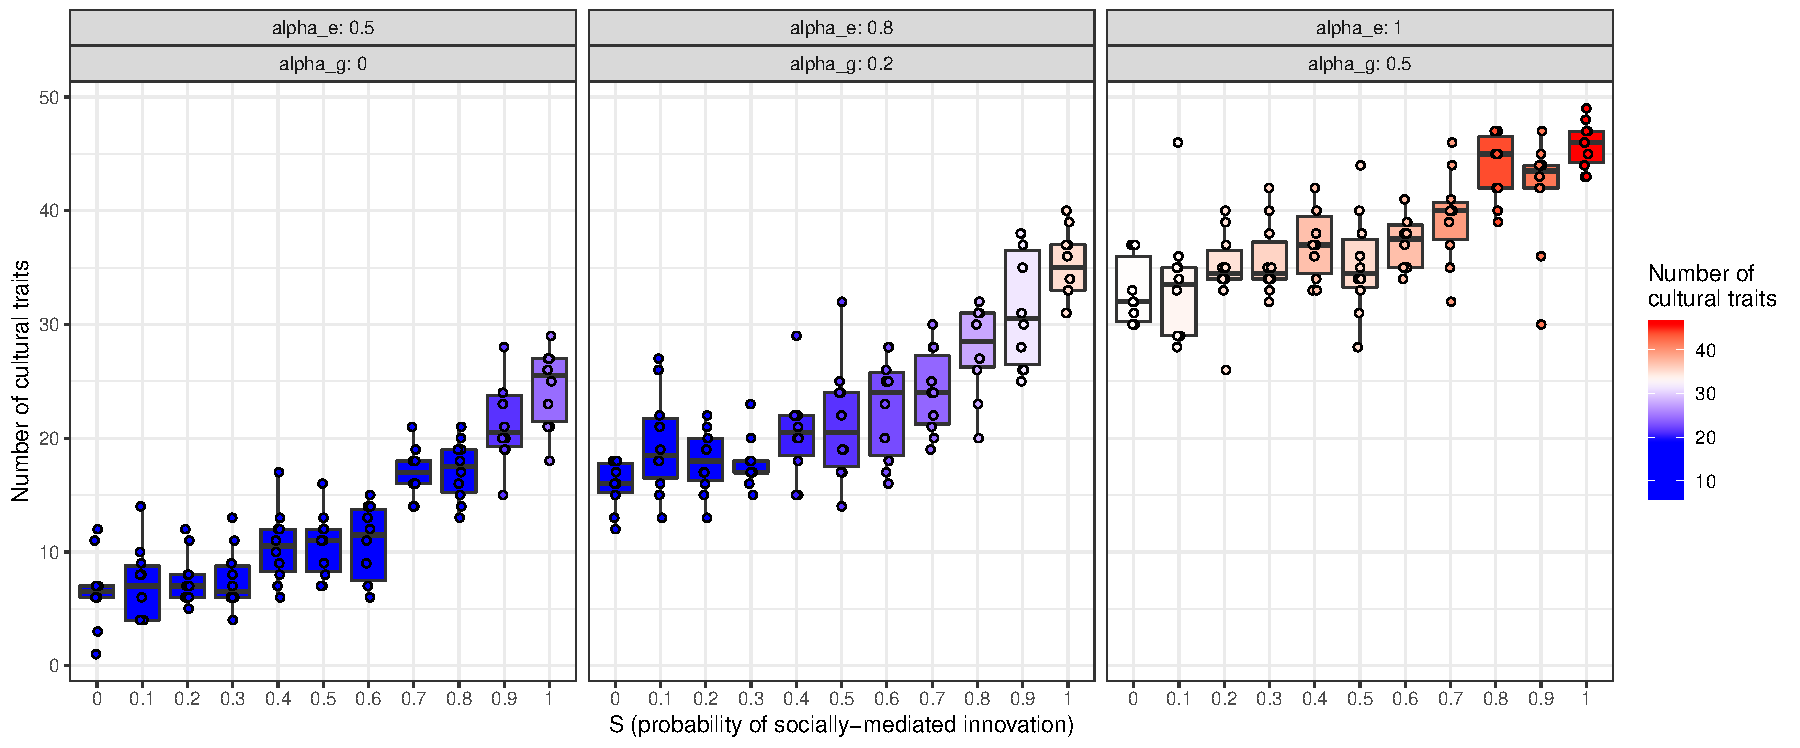
\includegraphics[width=11.4cm]{figures/figure_3.pdf}
\caption{Number of behaviours for each of the four patterns (*A*, *B*, *C*, *D*) for the parameters $\alpha_e=0.8;\alpha_g=0.2,S=1$. The red values are the values described for real chimpanzees populations.}
\label{Figure3}
\end{center}
\end{figure*}

Finally, we run 100 simulations for the same condition where we have a
good match for cultural behaviours with (1)
(\(\alpha_e=0.8;\alpha_g=0.2, S=1\)). In each simulation, we recorded,
for each population, the number of behaviours (habitual + customary +
present) that are also classified as cultural (see Figure
\ref{Figure4}). We find a weak but significant correlation b between
population size and number of cultural traits
(\(p<0.00001,\rho=0.2,N=600\)).

\begin{figure*}[h!]
\begin{center}
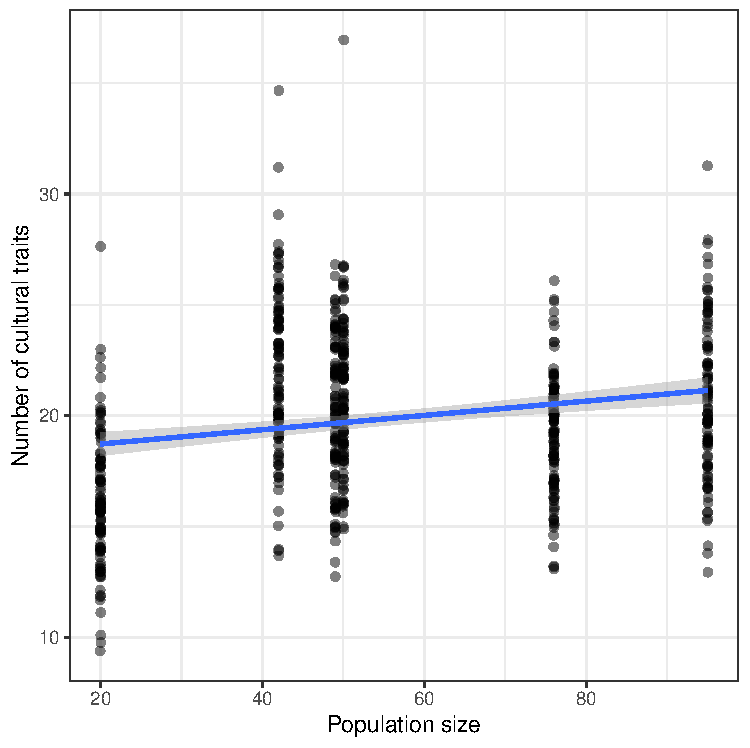
\includegraphics[width=11.4cm]{figures/figure_4.pdf}
\caption{Number of cultural behaviours for each population for the parameters $\alpha_e=0.8;\alpha_g=0.2,S=1$. The blue line is a linear fit of the data.}
\label{Figure4}
\end{center}
\end{figure*}

\section*{Discussion}\label{discussion}
\addcontentsline{toc}{section}{Discussion}

TO DO

\showmatmethods
\showacknow
\pnasbreak

\hypertarget{refs}{}
\hypertarget{ref-whiten_cultures_1999}{}
1. Whiten A, et al. (1999) Cultures in chimpanzees. \emph{Nature}
399(6737):682--685.

\hypertarget{ref-lind_number_2010}{}
2. Lind J, Lindenfors P (2010) The Number of Cultural Traits Is
Correlated with Female Group Size but Not with Male Group Size in
Chimpanzee Communities. \emph{PLoS ONE} 5(3).
doi:\href{https://doi.org/10.1371/journal.pone.0009241}{10.1371/journal.pone.0009241}.

\hypertarget{ref-wrangham_why_2000}{}
3. Wrangham RW (2000) Why are male chimpanzees more gregarious than
mothers? A scramble competition hypothesis. \emph{Primate Males: Causes
and Consequences of Variation in Group Composition} (Cambridge
University Press, Cambridge), pp 248--258.



% Bibliography
% \bibliography{pnas-sample}

\end{document}

